\documentclass[conference]{IEEEtran}
\usepackage{amsmath,amssymb}
\usepackage{graphicx}
\usepackage{booktabs}
\usepackage{xcolor}
\usepackage{url}
\usepackage[hidelinks]{hyperref}

% Numbers generated from the data by scripts/make_numbers.py
% generated by scripts/make_numbers.py -- do not edit by hand
\newcommand{\tExactWinterNSixteen}{5.1~min}
\newcommand{\degenWinterNSixteen}{1}
\newcommand{\tExactWinterNFourteen}{7.1~min}
\newcommand{\degenWinterNFourteen}{6}
\newcommand{\tExactWinterNEighteen}{49~min}
\newcommand{\degenWinterNEighteen}{2}
\newcommand{\exactSizesWinter}{14, 16, 18}
\newcommand{\SpeakWinter}{0.72}
\newcommand{\trotAWinter}{0.73}
\newcommand{\trotPWinter}{2.00}
\newcommand{\trotNptsWinter}{30}
\newcommand{\trotFreeAlphaWinter}{-0.12}
\newcommand{\classBaseWinter}{2.13}
\newcommand{\prepGapWinter}{0.37}
\newcommand{\prepKappaWinter}{0.21}
\newcommand{\NstarWinterA}{36}
\newcommand{\NstarFastHundredWinterA}{42}
\newcommand{\NstarFastTenThousandWinterA}{50}
\newcommand{\NstarPrepWinterA}{86}
\newcommand{\tQuantumWinterA}{23~yr}
\newcommand{\tClassicalWinterA}{54~yr}
\newcommand{\physQWinterA}{1.3\,M}
\newcommand{\gapNQMWinterA}{1345}
\newcommand{\gapQpiAIWinterA}{40}
\newcommand{\shotsWinter}{1752}
\newcommand{\circuitsWinterA}{7.3\times10^{4}}
\newcommand{\stepsWinterA}{396}
\newcommand{\rotPerStepWinterA}{862}
\newcommand{\NstarWinterB}{34}
\newcommand{\NstarFastHundredWinterB}{42}
\newcommand{\NstarFastTenThousandWinterB}{48}
\newcommand{\NstarPrepWinterB}{82}
\newcommand{\tQuantumWinterB}{9.7~yr}
\newcommand{\tClassicalWinterB}{12~yr}
\newcommand{\physQWinterB}{0.20\,M}
\newcommand{\gapNQMWinterB}{199}
\newcommand{\gapQpiAIWinterB}{400}
\newcommand{\circuitsWinterB}{6.9\times10^{4}}
\newcommand{\stepsWinterB}{396}
\newcommand{\rotPerStepWinterB}{814}
\newcommand{\NstarEpsOneWinterA}{42}
\newcommand{\NstarEpsOneWinterB}{40}
\newcommand{\dE}{0.50}
\newcommand{\epsPct}{5}
\newcommand{\Tmev}{17.5}
\newcommand{\Tps}{11.5}
\newcommand{\TroughPs}{8.3}
\newcommand{\nTimes}{169}
\newcommand{\omegaMax}{30}
\newcommand{\nqmMax}{1000}
\newcommand{\nqmMin}{50}
\newcommand{\qpiaiFid}{96}
\newcommand{\mainSet}{Winter}


% Red notes mark what the authors still have to check or decide.
% Every \verify must be resolved before submission (grep for it).
\newcommand{\verify}[1]{\textcolor{red}{[#1]}}
\newcommand{\RuCl}{$\alpha$-RuCl$_3$}
\newcommand{\eps}{\varepsilon}

\begin{document}

\title{When Will Quantum Computers Beat Classical Simulation of a Real Quantum Magnet?
A Quantum--Classical Crossover for the Neutron Spectrum of \RuCl}

\author{\IEEEauthorblockN{Anonymous Author(s)}
\IEEEauthorblockA{Proceedings Track submission}}

\maketitle

\begin{abstract}
Claims of quantum advantage for simulating materials are usually made for
toy models at an arbitrary accuracy. We ask the question for a real
material and an accuracy fixed by experiment: the dynamical structure
factor $S(\mathbf q,\omega)$ of the Kitaev magnet \RuCl, resolved to the
energy resolution of inelastic neutron scattering. We measure the cost of
exact classical simulation on clusters of up to 18 spins, measure the
Trotter error of the corresponding quantum circuits against the exact
results, and feed the logical circuits to a surface-code resource
estimator. Across \nSets{} published exchange models, a fault-tolerant
quantum computer overtakes exact state-vector simulation at
$N^*\approx\NstarRangeAll$ spins. For the \mainSet{} \emph{et al.}
model it needs \physQWinterB{} (\physQWinterA{}) physical qubits at a
physical error rate of $10^{-4}$ ($10^{-3}$), and at the crossover both
machines need about a century, so the crossover marks where neither is
practical rather than where quantum simulation becomes useful. Preparing
the ground state from the best product state moves the crossover to
$N^*\approx\NstarPrepRangeWinter$. The qubit count at $N^*$ exceeds the
1000-qubit target of India's National Quantum Mission by a factor of
\gapNQMWinterB--\gapNQMWinterA. We claim no advantage today;
every projection is stated with its assumptions, and code and data are
public.
\end{abstract}

\begin{IEEEkeywords}
quantum advantage, resource estimation, Kitaev materials, neutron scattering, Trotter error
\end{IEEEkeywords}

\noindent\textbf{Plain-language summary.}
Neutron beams reveal how the magnetic moments inside a crystal move, and
comparing those measurements with a model needs a computer simulation that
becomes exponentially harder as the simulated piece of crystal grows. We
estimate how large that piece must be before a future error-corrected
quantum computer would finish the job faster than a classical computer,
using the real accuracy of neutron experiments on the magnet \RuCl. The
answer is a few dozen magnetic atoms, but reaching it requires hundreds of
thousands of physical qubits, far beyond any machine built or planned so far.

\section{Introduction}

Simulating quantum dynamics is the application most often named for
quantum computers, yet most crossover studies cost a model Hamiltonian at an
accuracy chosen by the authors. Yoshioka \emph{et al.}~\cite{yoshioka2024}
located the quantum--classical crossover for ground-state energies of
two-dimensional model Hamiltonians, and Sun \emph{et
al.}~\cite{sun2026} did so for the dynamics of the mixed-field Ising model,
benchmarking against tensor-network and variational Monte Carlo methods.
Two ingredients are still missing for a statement a materials scientist
can use: a real material whose Hamiltonian is not exactly solvable, and an
accuracy target set by an actual measurement rather than by a free
parameter $\eps$.

\RuCl{} is the leading candidate for Kitaev's honeycomb spin
liquid~\cite{kitaev2006,jackeli2009,takagi2019}. Its inelastic neutron
scattering (INS) spectrum shows a continuum whose origin is debated
\cite{banerjee2016,banerjee2017,do2017,winter2017}, several exchange
models compete~\cite{winter2017,ran2017,laurell2020}, and exact
diagonalization on small clusters is the standard tool for comparing them
with data~\cite{laurell2020}. It is therefore a natural target for quantum
simulation, and a natural test of when that simulation would pay off.

\textbf{Contributions.} (i) An accuracy target derived from the INS energy
resolution: the time window, total simulated time and spectral tolerance
all follow from one measured number (Sec.~\ref{sec:target}). (ii) Measured
classical cost of exact time-domain simulation of $S(\mathbf q,\omega)$ on
periodic clusters, including the degenerate ground manifolds that
symmetric clusters carry (Sec.~\ref{sec:classical}). (iii) Trotter errors
measured on the experimental observable itself, for the exact circuit whose
gates are counted, and a full surface-code resource estimate with
ground-state preparation as a separate line item (Sec.~\ref{sec:quantum}).
(iv) The crossover $N^*$, its sensitivity, and the gap between the hardware
it needs and India's stated targets (Sec.~\ref{sec:results}).

\section{Model and accuracy target}\label{sec:target}

We use the spin-1/2 $J_1$--$K$--$\Gamma$--$\Gamma'$--$J_3$ model on the
honeycomb lattice~\cite{rau2014,winter2017},
\begin{multline}
H=\sum_{\langle ij\rangle_\gamma}\Big[J_1\,\mathbf S_i\!\cdot\!\mathbf S_j
+K S_i^\gamma S_j^\gamma
+\Gamma\big(S_i^\alpha S_j^\beta+S_i^\beta S_j^\alpha\big)\\
+\Gamma'\!\!\sum_{\mu=\alpha,\beta}\!\big(S_i^\gamma S_j^\mu+S_i^\mu S_j^\gamma\big)\Big]
+J_3\!\!\sum_{\langle\langle\langle ij\rangle\rangle\rangle}\!\!\mathbf S_i\!\cdot\!\mathbf S_j,
\end{multline}
where $\gamma\in\{x,y,z\}$ labels the bond and $\alpha,\beta$ the other two
axes. Our main set is that of Winter \emph{et al.}~\cite{winter2017},
$(J_1,K,\Gamma,J_3)=(-0.5,-5.0,2.5,0.5)$\,meV
\verify{check values and convention against the paper}; the
$K$--$\Gamma$ model of Ran \emph{et al.}, $(K,\Gamma)=(-6.8,9.5)$\,meV~\cite{ran2017},
and the set used by Laurell and Okamoto~\cite{laurell2020},
$(J_1,K,\Gamma,\Gamma',J_3)=(-1.3,-15.1,10.1,-0.12,0.9)$\,meV
\verify{check which of their models this is}, test the sensitivity to the
model; their energy scales are about two and three times larger.

\textbf{Observable.} We compute
\begin{equation}
S(\mathbf q,\omega)=\frac{1}{2\pi}\!\int_{-T}^{T}\!\!dt\,w(t)\,e^{i\omega t}
\frac1N\sum_{ij}e^{i\mathbf q\cdot(\mathbf r_i-\mathbf r_j)}
\langle\mathbf S_i(t)\!\cdot\!\mathbf S_j(0)\rangle
\end{equation}
($\hbar=1$, energies in meV). An instrument with Gaussian resolution of
full width $\delta E$ measures the true spectrum convolved with that
Gaussian, which in the time domain is \emph{exactly} the window
$w(t)=e^{-t^2/2\tau^2}$ with $\tau=2\sqrt{2\ln2}/\delta E$. The
correlation function is therefore needed only up to the time
$T=\tau\sqrt{2\ln(1/c)}$ at which the window falls below a cutoff $c$
(we use $c=10^{-3}$), and sampling at $\Delta t=\pi/\omega_{\max}$ resolves
energies up to $\omega_{\max}=\omegaMax$\,meV. For $\delta E=\dE$\,meV
\verify{take $\delta E$ from \cite{banerjee2017,do2017}} this gives
$T=\Tmev$\,meV$^{-1}=\Tps$\,ps (the rough estimate $2\pi\hbar/\delta E$
gives \TroughPs\,ps) and \nTimes{} time points. We demand that the
resolution-convolved spectrum $\sum_a S^{aa}(\mathbf q,\omega)$ be correct to
$\eps=\epsPct\%$ of its peak value \verify{set $\eps$ below the
experimental error bars}, split equally between Trotter error and shot
noise.

\begin{figure}[t]
\centering
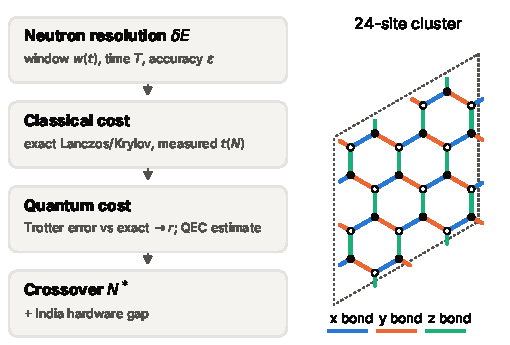
\includegraphics[width=\columnwidth]{../figures/fig1_pipeline.pdf}
\caption{The pipeline: the neutron resolution fixes the window, the total
time and the accuracy; classical and quantum costs are measured or
estimated for the same target and meet at $N^*$. Right: a 24-site periodic
cluster with Kitaev bond labels (open and filled circles are the two
sublattices; stubs leave the cell and re-enter on the opposite side).}
\label{fig:pipeline}
\end{figure}

\section{Classical cost}\label{sec:classical}

\textbf{Clusters.} For each $N$ we enumerate all periodic supercells of
$N/2$ unit cells by their Hermite normal forms and take the most compact
one on which every nearest- and third-neighbour bond maps to a distinct
pair of sites. Third-neighbour bonds are faithful only for $N\ge14$, so we
use $N=\exactSizesWinter$ here; $N=20$ and $24$ are run separately
\verify{add $N=20, 24$ results}.

\textbf{Method.} The model has no $U(1)$ symmetry, so we work in the full
$2^N$-dimensional space with a matrix-free Hamiltonian. The ground state is
found by two-pass Lanczos; symmetric clusters have degenerate ground
levels (\degenWinterNFourteen-fold for $N=14$, matching three zigzag
orientations times time reversal, and \degenWinterNEighteen-fold for $N=18$
with the \mainSet{} parameters), which we resolve by deflated Lanczos and
average over, since a single Lanczos vector breaks translation symmetry. Each $S_j^b|0\rangle$ is propagated by
short-iterative Lanczos~\cite{park1986} with an a-posteriori error bound
of $10^{-9}$, and overlaps with $S_i^a$ give all correlators at each
time; translation invariance reduces the reference sites $j$ to one per
sublattice. The code is checked against the exactly solvable Kitaev
limit~\cite{kitaev2006,baskaran2007} (conserved plaquettes, ultra-short-ranged
static and dynamical correlations, ground-state energy within 2\% of the
thermodynamic value) and against the exact Lehmann sum for $N=8$, which
the time-domain result matches to $10^{-4}$ of the peak.

\textbf{Measured cost.} The full spectrum takes \tExactWinterNFourteen,
\tExactWinterNSixteen{} and \tExactWinterNEighteen{} on a 4-core
workstation for $N=14,16,18$ (all ground states included). Per ground
state, the cost follows $t\propto N^2 2^N$ (matrix--vector cost $\propto
N2^N$ times a number of products $\propto\|H\|T\propto NT$); a free
exponential fit gives a base of \classBaseWinter. Fig.~\ref{fig:spectrum}
shows the computed spectrum for $N=18$.

\begin{figure}[t]
\centering
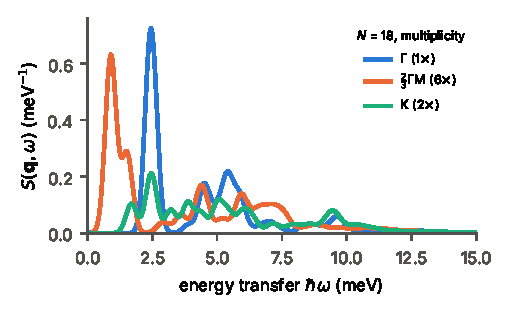
\includegraphics[width=\columnwidth]{../figures/fig2_spectrum_winter2017_N18.pdf}
\caption{Computed $\sum_a S^{aa}(\mathbf q,\omega)$ at the symmetry-distinct
momenta of the 18-site cluster (\mainSet{} parameters), convolved with the
resolution $\delta E=\dE$\,meV. Legend: momentum and number of equivalent
momenta. \verify{replace by $N=24$ once run}}
\label{fig:spectrum}
\end{figure}

\section{Quantum cost}\label{sec:quantum}

\textbf{Circuit.} One qubit per spin plus one ancilla. Each correlator is
measured by the Hadamard test with controlled Paulis and an
\emph{uncontrolled} evolution between them~\cite{somma2002}, so the
evolution circuit is the only non-Clifford part. The evolution is a
second- or fourth-order Suzuki product formula~\cite{suzuki1991} over the
Pauli strings of $H$: five rotations $e^{-i\theta\sigma^a_i\sigma^b_j}$ per
nearest-neighbour bond for the \mainSet{} set (nine if $\Gamma'\neq0$) and
three per third-neighbour bond, ordered by bond family, with neighbouring
rotations about the same string fused.

\textbf{Trotter error, measured.} We simulate exactly this rotation
sequence on a state vector, form the correlators as the Hadamard test
would (evolving both $|0\rangle$ and $S^b_j|0\rangle$ with the circuit),
and compute the error of the resolution-convolved spectrum against the
exact result for $N=\exactSizesWinter$, several step sizes $\delta t$ and
three resolutions. The data follow $\eps_{\rm Trot}=A\,T\,\delta t^{p}$ with
$p=\trotPWinter$ for second order (\trotNptsWinter{} points); fitting an
explicit $N^\alpha$ gives $\alpha=\trotFreeAlphaWinter$, so we take the
largest prefactor among the measured sizes, $A=\trotAWinter$, and no growth
with $N$. This is the expected behaviour for an intensive,
resolution-limited quantity; commutator bounds~\cite{childs2021} would be
far more pessimistic.

\textbf{Shots.} Each shot gives $\pm1$, so the variance of a correlator of
spin-1/2 operators is at most $1/16n$ after $n$ shots. Propagating this
through the windowed transform gives
$\mathrm{Var}\,S\le 3N\sum_k (w_k\Delta t)^2/(32\pi^2 n)$, and we choose $n$
so that two standard deviations stay below half of $\eps S_{\max}$.
Here $S_{\max}$ is the peak of the inelastic spectrum ($\omega>2\delta E$),
excluding the quasi-elastic weight that piles up at the zigzag ordering
vector on clusters that fit that order, and taking the smallest peak over
the measured sizes ($S_{\max}=\SpeakWinter$\,meV$^{-1}$ for the
\mainSet{} set, $n\approx\shotsWinter$). With one reference site per sublattice, three
spin components and real and imaginary parts, $12N$ circuits are needed per
time point, $\circuitsWinterA$ in total at $N=\NstarWinterA$. All are
independent, so they could run on many machines at once; we compare one
quantum computer with one classical workstation.

\textbf{Error correction.} Logical counts (qubits, rotations, rotation
depth from as-soon-as-possible scheduling) are passed to Microsoft's
resource estimator~\cite{beverland2022} with a surface code~\cite{fowler2012},
gate-based qubits with nanosecond gate times and physical error rates
$p=10^{-3}$ and $10^{-4}$, and a total error budget of 1\% per circuit;
rotation synthesis~\cite{ross2016} and magic-state factories are included
by the estimator. One machine runs all circuits sequentially.

\textbf{Ground-state preparation.} We use a simple model of
phase-estimation projection from a product state with overlap $\gamma$:
an evolution time $2\pi\ln(1/\delta)/\Delta$ per attempt with controlled
evolution at twice the cost, and $1/\gamma^2$ attempts per shot;
near-optimal methods reduce the latter to $1/\gamma$~\cite{lin2020}. From exact
results we take the mean gap $\Delta=\prepGapWinter$\,meV and the best
product-state overlap, optimised over all single-spin directions, which
decays as $\gamma\propto e^{-\prepKappaWinter N}$ over $N=\exactSizesWinter$.
This line item is reported separately because it is the least certain.

\section{Crossover and India roadmap}\label{sec:results}

\begin{figure}[t]
\centering
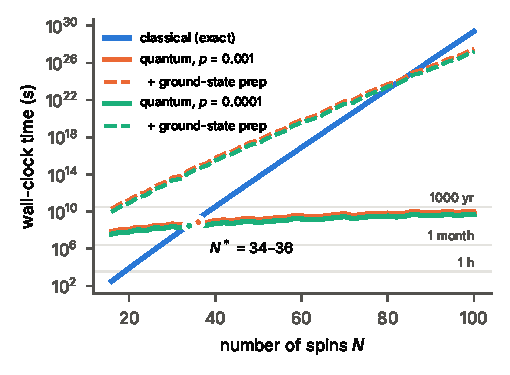
\includegraphics[width=\columnwidth]{../figures/fig3_crossover_winter2017.pdf}
\caption{Wall-clock time to obtain $S(\mathbf q,\omega)$ at the
experimental resolution and accuracy, against the number of spins.
Classical: exact simulation, measured for $N\le18$ and extrapolated as
$N^22^N$. Quantum: second-order Trotter circuits, surface code, without
(solid) and with (dashed) ground-state preparation.}
\label{fig:crossover}
\end{figure}

\begin{table}[t]
\centering
\caption{Fault-tolerant resources at the crossover for the three
parameter sets (second-order Trotter, $\delta E=\dE$\,meV,
$\eps=\epsPct\%$). $r$: Trotter steps for the longest time; $d$: code
distance; runtime excludes ground-state preparation.}
\label{tab:resources}
\footnotesize
\setlength{\tabcolsep}{3.2pt}
% generated by scripts/make_numbers.py -- do not edit by hand
\begin{tabular}{@{}lccccccc@{}}
\toprule
Set & $p$ & $N^*$ & $r$ & T states & $d$ & Phys.\ qubits & Runtime \\
 & & & (steps) & per shot & & & at $N^*$ \\
\midrule
Winter & $10^{-3}$ & 36 & 396 & $6.5\times10^{6}$ & 19 & $1.3$\,M & 23~yr \\
Winter & $10^{-4}$ & 34 & 396 & $6.1\times10^{6}$ & 9 & $0.20$\,M & 9.7~yr \\
Ran & $10^{-3}$ & 36 & 1757 & $1.1\times10^{7}$ & 19 & $5.2$\,M & 25~yr \\
Ran & $10^{-4}$ & 34 & 1757 & $1.1\times10^{7}$ & 9 & $0.40$\,M & 11~yr \\
\bottomrule
\end{tabular}

\end{table}

Fig.~\ref{fig:crossover} shows the result for the \mainSet{} set. The
quantum cost grows only polynomially, but its prefactor is large: at $N^*$
a single circuit runs for seconds, and $\sim10^5$ circuits each need
$\sim10^4$ shots. The curves cross at $N^*=\NstarRangeWinter$ for both
error rates, where the quantum computer needs \tQuantumWinterB{}
($p=10^{-4}$) or \tQuantumWinterA{} ($p=10^{-3}$) against
\tClassicalWinterB{} classically (Table~\ref{tab:resources}). The
crossover is therefore a statement about scaling, not about a useful
computation: practical simulation at $N^*$ needs both far more parallel
hardware and better algorithms on each side. Fourth-order formulas give
the same $N^*$, because fewer steps are offset by five times as many
rotations per step. Including ground-state preparation moves the
crossover to $N^*=\NstarPrepRangeWinter$, because the product-state
overlap shrinks exponentially; better initial states~\cite{lin2020} are
the main lever.

\textbf{Sensitivity.} \emph{Accuracy:} $\eps=1\%$ instead of
\epsPct\% moves $N^*$ to \NstarEpsOneRangeWinter. \emph{Classical
hardware:} a classical machine $10^2$ or $10^4$ times faster than our
workstation, such as a large cluster, moves it to
\NstarFastHundredRangeWinter{} and \NstarFastTenThousandRangeWinter: each
factor of two in classical speed costs roughly one spin. \emph{Model:}
the Ran \emph{et al.} and Laurell--Okamoto sets (exact data for
$N=\exactSizesRan$) have Trotter prefactors $A=\trotARan$ and
\trotALaurell, twenty to thirty times that of the \mainSet{} set, and need
\stepsRanA{} and \stepsLaurellA{} instead of \stepsWinterA{} steps, yet
they cross over at $N^*=\NstarRangeRan$ and \NstarRangeLaurell: the step
count grows only as $A^{1/2}$, and the circuit and shot counts, which
dominate, barely change. Longer circuits need more magic-state factories,
so at $p=10^{-3}$ these sets need \physQRanA{} and \physQLaurellA{}
physical qubits (Table~\ref{tab:resources}). With only two sizes the
overlap trend of these sets is not determined (for Laurell--Okamoto it
even rises from $N=14$ to $16$), so we do not quote their crossover with
ground-state preparation.

\begin{figure}[t]
\centering
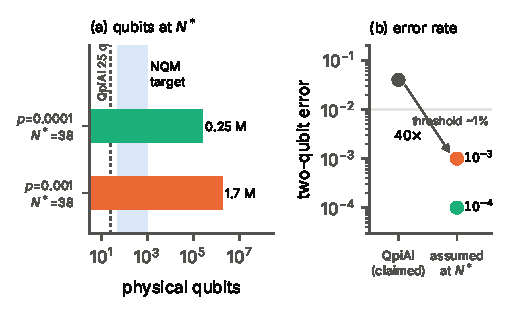
\includegraphics[width=\columnwidth]{../figures/fig4_india_winter2017.pdf}
\caption{(a) Physical qubits needed at $N^*$ against the National Quantum
Mission target of 50--1000 physical qubits~\cite{nqm2023} and the 25-qubit
QpiAI-Indus system~\cite{qpiai2025}. (b) The assumed physical error rates
against the reported two-qubit error of QpiAI-Indus.}
\label{fig:india}
\end{figure}

\textbf{India roadmap.} The National Quantum Mission aims at intermediate
scale machines with 50--1000 physical qubits within eight
years~\cite{nqm2023}. At $N^*$ we need \physQWinterB{} qubits at
$p=10^{-4}$ and \physQWinterA{} at $p=10^{-3}$, i.e.\ \gapNQMWinterB--\gapNQMWinterA{}
times the mission's upper target (Fig.~\ref{fig:india}). The reported 96\%
two-qubit fidelity of QpiAI-Indus~\cite{qpiai2025} corresponds to an
error of 4\%, above the $\sim$1\% surface-code threshold and
\gapQpiAIWinterA--\gapQpiAIWinterB{} times the error rates assumed here.
Both gaps must close for this application; the error-rate gap comes first,
because below threshold every further factor of ten in $p$ cuts the qubit
count roughly sixfold (Table~\ref{tab:resources}).

\section{Limitations and outlook}

\emph{Classical baseline.} Exact simulation is the weakest credible
classical method, so our $N^*$ is a lower bound on where advantage could
begin. Translation symmetry would save a further factor $\sim N/2$ and
continued-fraction Lanczos~\cite{gagliano1987} avoids time stepping
altogether for a fixed broadening; matrix-product-state time
evolution~\cite{haegeman2016,hauschild2018} on cylinders, PEPS,
time-dependent variational Monte Carlo and neural quantum states were not
run. Each could push $N^*$ up; long-time dynamics in two dimensions is
where they struggle most. \emph{Extrapolation.} Classical costs and Trotter errors are
extrapolated from $N\le18$ (\mainSet{}) or $N\le16$ (the other sets); the
absence of an $N$ trend in the Trotter error rests on few sizes with strong
finite-size effects, and so does the reference peak $S_{\max}$, which
varies by a factor of three between sizes. \emph{Measurement.} Measuring $S(\mathbf q,t)$ directly rather
than site-resolved correlators, or sharing shots between circuits, could
cut the circuit count by up to a factor $N$. \emph{Physics.} We assume zero
temperature, ignore the neutron polarization factor and use parameter sets
that are themselves uncertain. \emph{Ground-state preparation} is modelled
coarsely and dominates when included. Despite these caveats, the
experiment-defined target turns ``quantum advantage for materials'' into a
concrete, checkable number, and our open code lets each assumption be
replaced.

\textbf{Code and data.} \url{https://anonymous.4open.science/r/XXXX}
\verify{create the anonymous mirror}.

\verify{AI-assistance disclosure if required by SQST/IEEE policy.}

\bibliographystyle{IEEEtran}
\bibliography{refs}

\end{document}
